\documentclass[10pt]{article}
\usepackage[usenames, dvipsnames]{xcolor}

\usepackage[utf8]{inputenc}
\usepackage{tikz}
\usetikzlibrary{positioning, calc, arrows, arrows.meta, fit, backgrounds, shapes, snakes}
\usepackage{graphicx}
\usepackage{amssymb}
\usepackage{amsmath}
\usepackage{amsfonts}

\newcommand{\yhat}{\hat{\V{y}}}
\newcommand{\ycorrect}{\hat{y}^+}
\newcommand{\thetadelta}{\V{\Theta}_\delta}
\newcommand{\biasdelta}{b_\delta}
\newcommand{\biasclass}{\V{b}_\text{c}}
\newcommand{\thetaclass}{\V{\Theta}_\text{c}}
\newcommand{\thetafeat}{\V{\Theta}_\text{feat}}
\newcommand{\fclass}{f_\text{c}}
\newcommand{\fdelta}{f_\delta}
\newcommand{\ffeat}{f_\text{feat}}
\newcommand{\f}{f}

\newcommand{\rvtime}{T_c}
\newcommand{\xuptot}{\M{X}_{\rightarrow t}}
\newcommand{\deltauptot}{\delta_{\rightarrow t}}
\newcommand{\tstop}{\ensuremath{s_t}}
\newcommand{\meantstop}{earliness}
\newcommand{\ptoffset}{\ensuremath{\varepsilon}}
\newcommand{\deltat}{p_\text{dec}(\xuptot)}%{p_t}%\delta_t
\newcommand{\Pt}{\ensuremath{P_t}} % P(t)
\newcommand{\pt}{\deltat}
\newcommand{\PT}{\ensuremath{P_T}}
\newcommand{\Puptot}{\ensuremath{P_{\rightarrow t}}} % \mathcal{B}_{t-1}
\newcommand{\PuptoT}{\ensuremath{P_{\rightarrow T}}} % \mathcal{B}_{t-1}

\definecolor{colororange}{HTML}{E65100} % orange
\definecolor{colordgray}{HTML}{795548} % dark gray for note
\definecolor{colorhgray}{HTML}{212121} % heavy dark gray for normal text
\definecolor{colorblue}{HTML}{009688} % green
\definecolor{colorlgray}{HTML}{FFFFFF} % FAFAFA background light gray

\tikzstyle{rnn}=[draw,circle]
\tikzstyle{annot}=[rounded corners]
\tikzstyle{infer}=[-stealth, shorten >=.0em, shorten <=.0em]
\tikzstyle{loss}=[fill=colordgray!10, rounded corners, font=\small]
\tikzstyle{grad}=[]


\begin{document}
\pagestyle{empty}

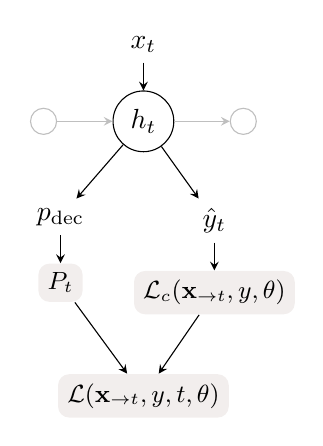
\begin{tikzpicture}[node distance=1em and .8em]
\node[](x0){$x_t$};
\node[rnn, below=of x0](h0){$h_t$};  %$\theta_\text{rnn}$};
\node[below right= 2em and 1em of h0](y0){$\hat{y}_t$};
\node[rnn, left=2em of h0,draw=lightgray](hprev){};
\node[rnn, right=2em of h0,draw=lightgray](hnext){};
\node[below left= 2em and 1em of h0](d0){$p_\text{dec}$};

\node[loss, below=of y0](L0){$\mathcal{L}_c (\mathbf{x}_{\rightarrow t}, y, \theta)$};
%\node[right=of L0](t0){$\V{y}_t$};
\draw[-stealth, grad] (y0) -- (L0);
%\draw[-stealth, grad] (t0) -- (L0);

\draw[infer] (x0) -- (h0);
\draw[infer,draw=lightgray] (hprev) -- (h0);
\draw[infer,draw=lightgray] (h0) -- (hnext);
\draw[infer] (h0) -- (y0) node[midway,right, text=black](wc){};
\draw[infer] (h0) -- (d0) node[midway,left, text=black](wd){};

\node[below=of d0, loss](pt){$\Pt$};
\node[below=8em of h0, loss](L){$\mathcal{L}(\mathbf{x}_{\rightarrow t}, y, t, \theta)$}; % = P(t)\mathcal{L}_c (\xuptot, y)$};

% \node[left=.5em of pt, loss](budget){$P_{\rightarrow t}$};

\draw[infer] (L0) -- (L);
\draw[infer] (d0) -- (pt);
\draw[infer] (pt) -- (L);
% \draw[infer] (budget) -- (pt);

\end{tikzpicture}


\end{document}
